

\subsection{Mejoras en del perfilador}
\begin{frame}{Mejoras en las mecánica del perfilador}
    \begin{onlyenv}<1>
        
    
    Primera iteración mecánica
    \begin{columns}[c]
        \begin{column}{0.4\textwidth}
            \begin{itemize}
                \item Facil colocación a la mesa óptica. 
                \item Motor encastrado en soporte. 
                \item Tamaño imposibilita usarlo en altura y otro eje
            \end{itemize}
        \end{column}
        \begin{column}{0.6\textwidth}
            \begin{figure}
                \centering
                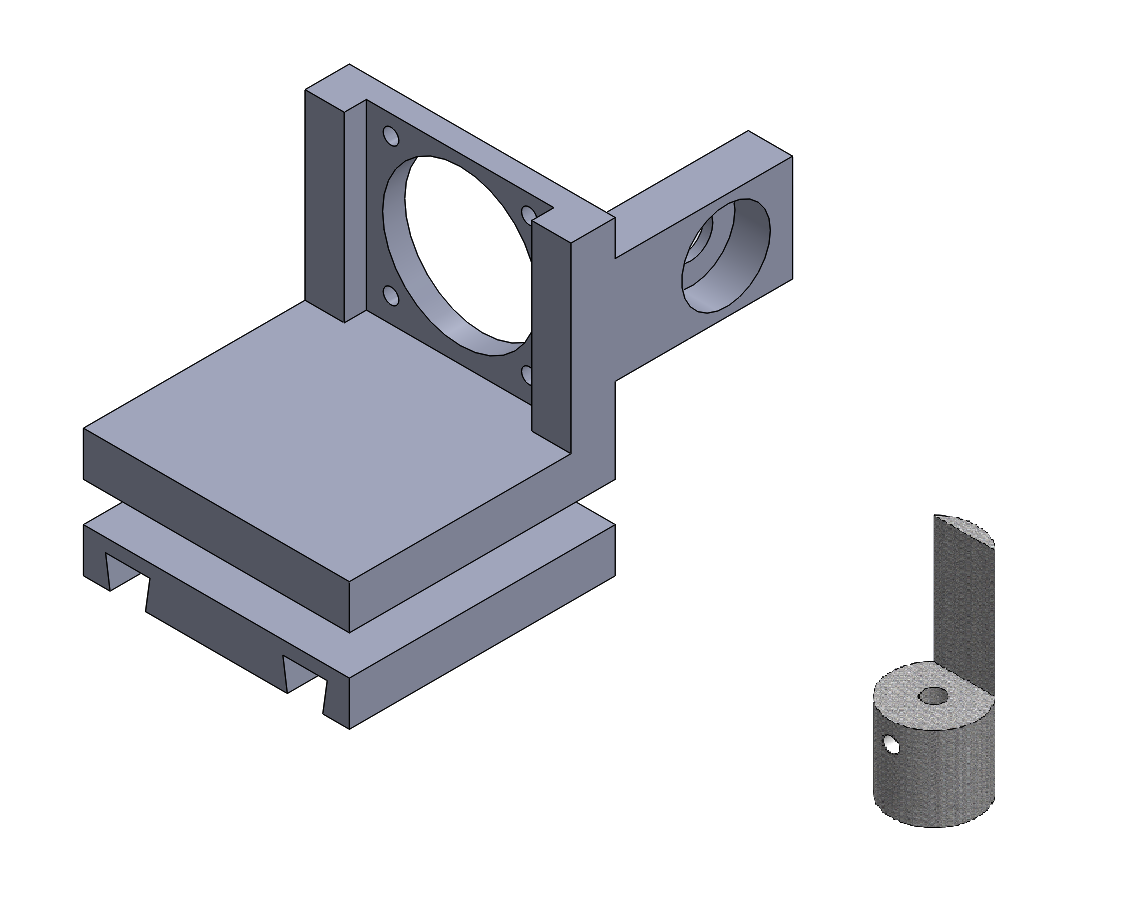
\includegraphics[width=\textwidth]{fig/perfilador/soporte_labo7_1}
             
                \label{fig:soporte_labo7}
            \end{figure}
        \end{column}
    \end{columns}
    \end{onlyenv}
    \begin{onlyenv}<2>
        
    Segunda iteración mecánica.
    \begin{columns}[c]
        \begin{column}{0.4\textwidth}
            \begin{figure}
                \centering
                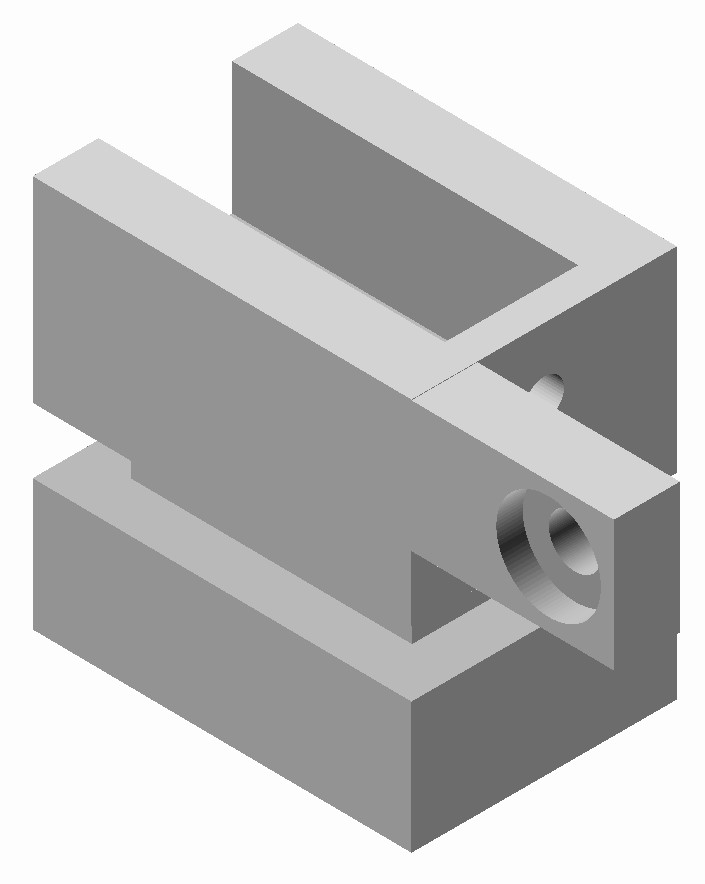
\includegraphics[width=0.8\textwidth]{fig/perfilador/soporte_labo7_2}
             
                \label{fig:soporte_labo7}
            \end{figure}
        \end{column}
        \begin{column}{0.5\textwidth}
            \begin{itemize}
                \item  Motor NEMA 8 de torque suficiente
                \item  Ubicable en altura y en otro eje
            \end{itemize}
            
        \end{column}
    \end{columns}
    \end{onlyenv}
\end{frame}

